\documentclass[10pt,pdf,hyperref={unicode}]{beamer}


%\documentclass[10pt]{beamer}

\usetheme[progressbar=frametitle]{metropolis}

\usepackage{booktabs}
\usepackage[scale=2]{ccicons}

\usepackage{pgfplots}

\usepgfplotslibrary{dateplot}

\usepackage{xspace}
\newcommand{\themename}{\textbf{\textsc{metropolis}}\xspace}

\usepackage{multicol}
%\usepackage{lmodern}

% подключаем кириллицу 
\usepackage[T2A]{fontenc}
\usepackage[utf8]{inputenc}
\usepackage{listings}
%\usepackage{graphicx}
\usepackage{hyperref}

% отключить клавиши навигации
\setbeamertemplate{navigation symbols}{}

% тема оформления
\usetheme{Pittsburgh}

% цветовая схема
\usecolortheme{default}

\definecolor{light-gray}{gray}{0.90}

\title{Семинар №11}   
\subtitle{ФАКТ \the\year}
\author{Бирюков В. А.} 
\date{\today}
% \logo{
\includegraphics[height=5mm]{images/logo.png}\vspace{-7pt}}

\begin{document}

\lstset{language=C}

% титульный слайд
\begin{frame}
\titlepage
\end{frame} 

\lstset{
  language=C,                % choose the language of the code
  basicstyle=\linespread{1.1}\ttfamily,
  columns=fixed,
  fontadjust=true,
  basewidth=0.5em,
  keywordstyle=\color{blue}\bfseries,
  commentstyle=\color{gray},
  stringstyle=\ttfamily\color{orange!50!black},
  showstringspaces=false,
  numbersep=5pt,
  numberstyle=\tiny\color{black},
  numberfirstline=true,
  stepnumber=1,                   % the step between two line-numbers.        
  numbersep=10pt,                  % how far the line-numbers are from the code
  backgroundcolor=\color{black!2},  % choose the background color. You must add \usepackage{color}
  showstringspaces=false,         % underline spaces within strings
  captionpos=b,                   % sets the caption-position to bottom
  breaklines=true,                % sets automatic line breaking
  breakatwhitespace=true,         % sets if automatic breaks should only happen at whitespace
  xleftmargin=.2in,
  extendedchars=\true,
  keepspaces = true,
}
\lstset{literate=%
   *{0}{{{\color{red!20!violet}0}}}1
    {1}{{{\color{red!20!violet}1}}}1
    {2}{{{\color{red!20!violet}2}}}1
    {3}{{{\color{red!20!violet}3}}}1
    {4}{{{\color{red!20!violet}4}}}1
    {5}{{{\color{red!20!violet}5}}}1
    {6}{{{\color{red!20!violet}6}}}1
    {7}{{{\color{red!20!violet}7}}}1
    {8}{{{\color{red!20!violet}8}}}1
    {9}{{{\color{red!20!violet}9}}}1
}

\newcommand{\imageSizeMult}{1.1}

\section{Бинарное дерево поиска}





\section{Добавление элемента в бинарное дерево поиска}

\begin{frame}[fragile]
\frametitle{Добавление элемента в бинарное дерево поиска}
Попробуем добавить элемент \texttt{50} в следующее дерево поиска:
\begin{center}
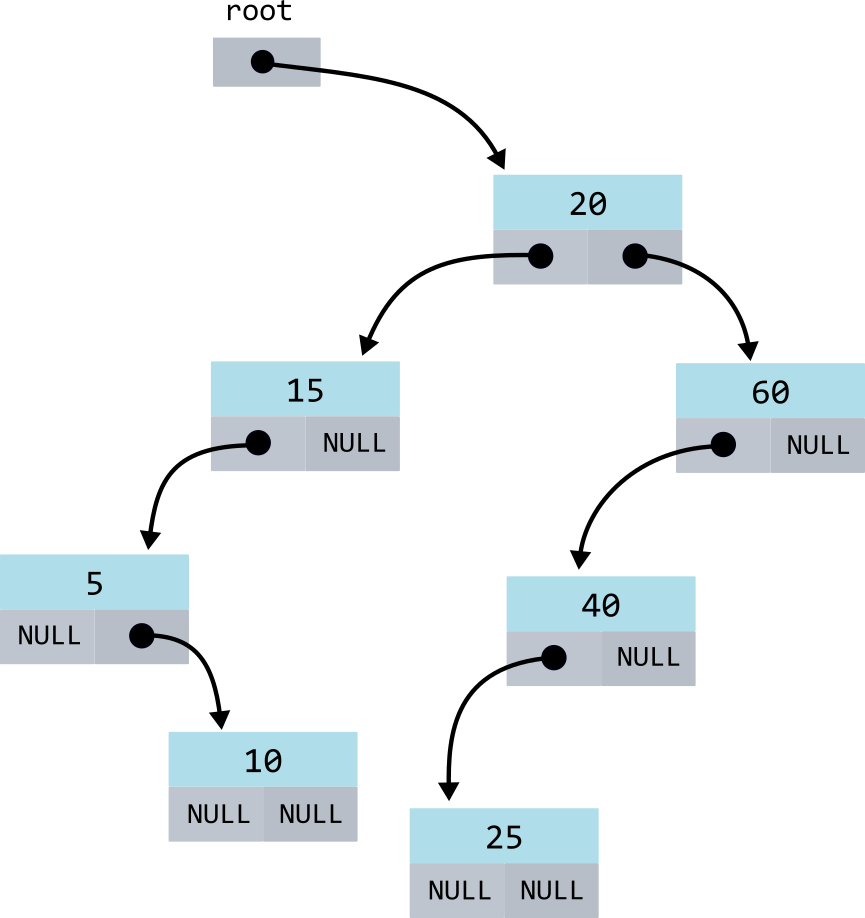
\includegraphics[width=0.5\linewidth]{../images/codetree/codetree0.png}
\end{center}
\end{frame}

\begin{frame}[fragile]
\frametitle{Добавление элемента в бинарное дерево поиска}
\begin{center}
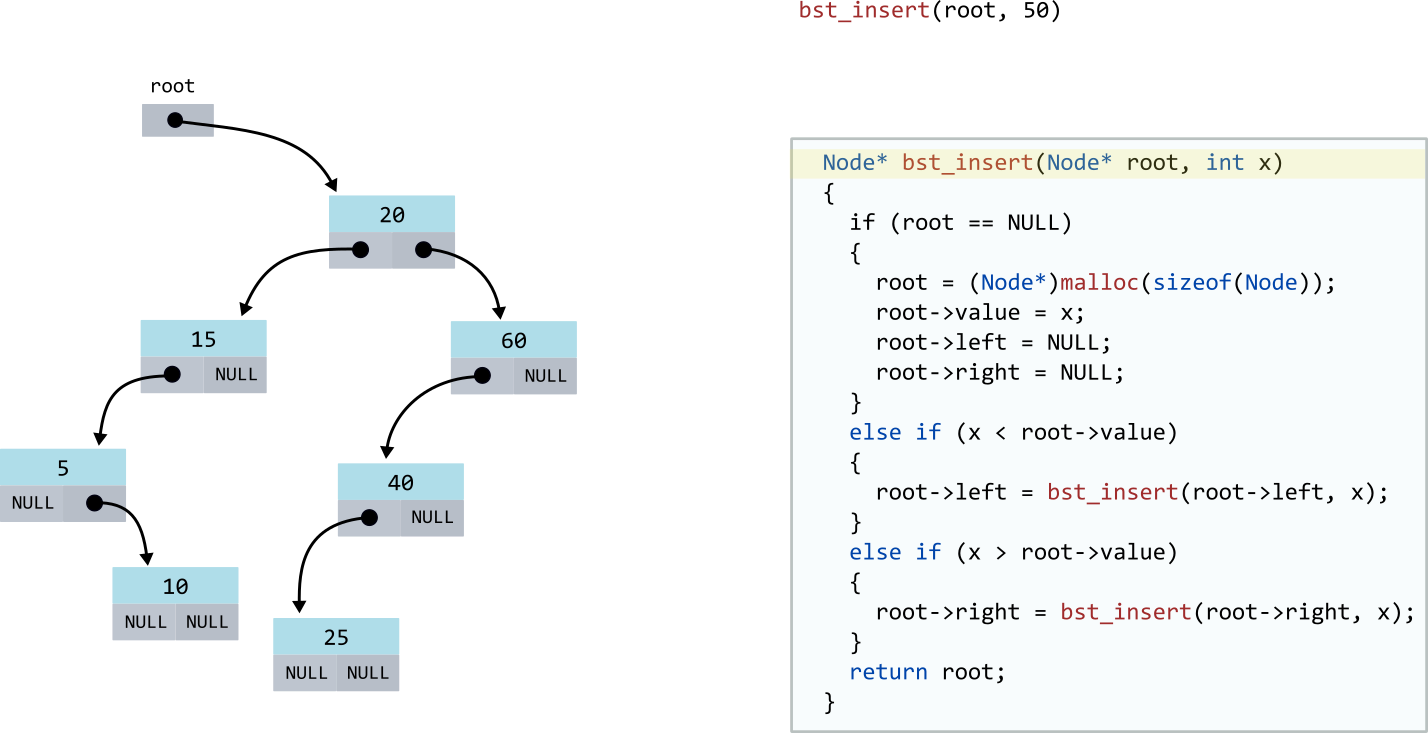
\includegraphics[width=\imageSizeMult\linewidth]{../images/codetree/codetree1.png}
\end{center}
\end{frame}

\begin{frame}[fragile]
\frametitle{Добавление элемента в бинарное дерево поиска}
\begin{center}
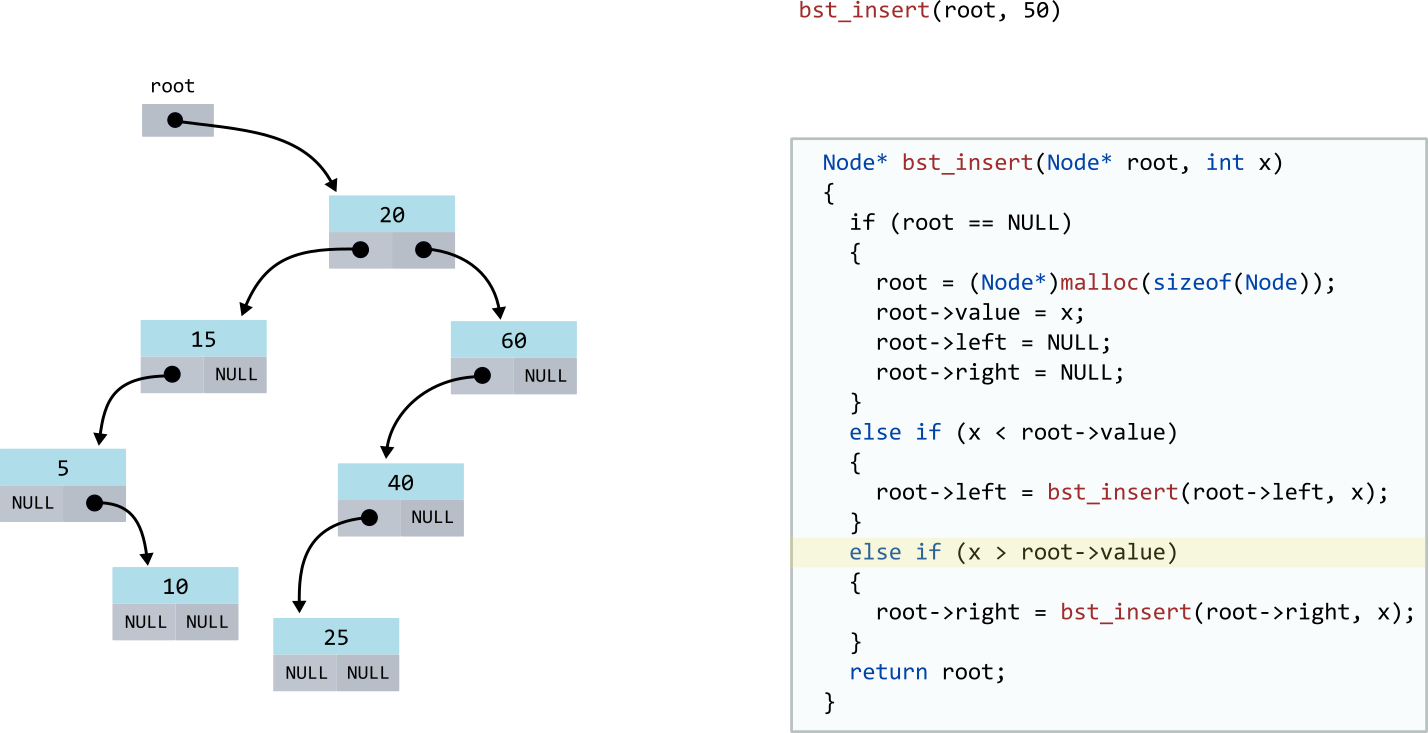
\includegraphics[width=\imageSizeMult\linewidth]{../images/codetree/codetree2.png}
\end{center}
\end{frame}

\begin{frame}[fragile]
\frametitle{Добавление элемента в бинарное дерево поиска}
\begin{center}
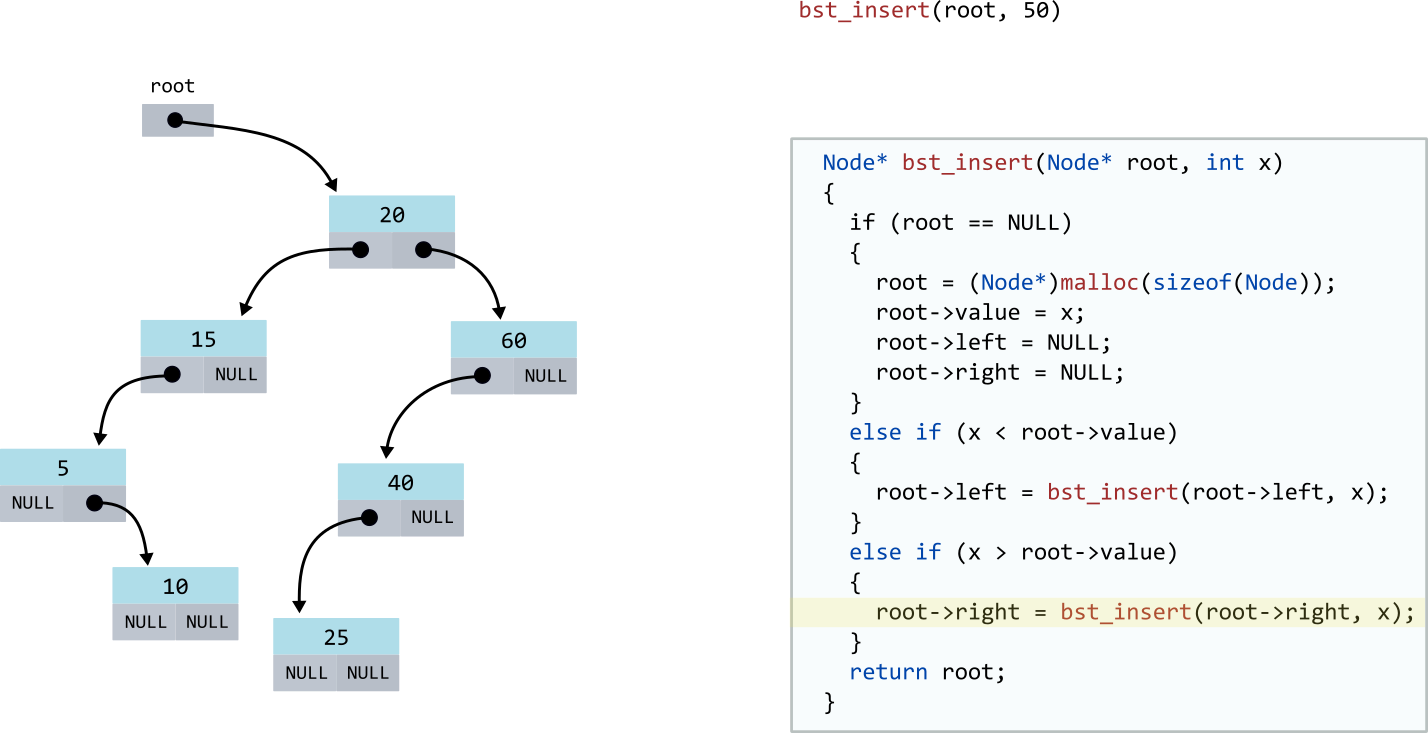
\includegraphics[width=\imageSizeMult\linewidth]{../images/codetree/codetree3.png}
\end{center}
\end{frame}

\begin{frame}[fragile]
\frametitle{Добавление элемента в бинарное дерево поиска}
\begin{center}
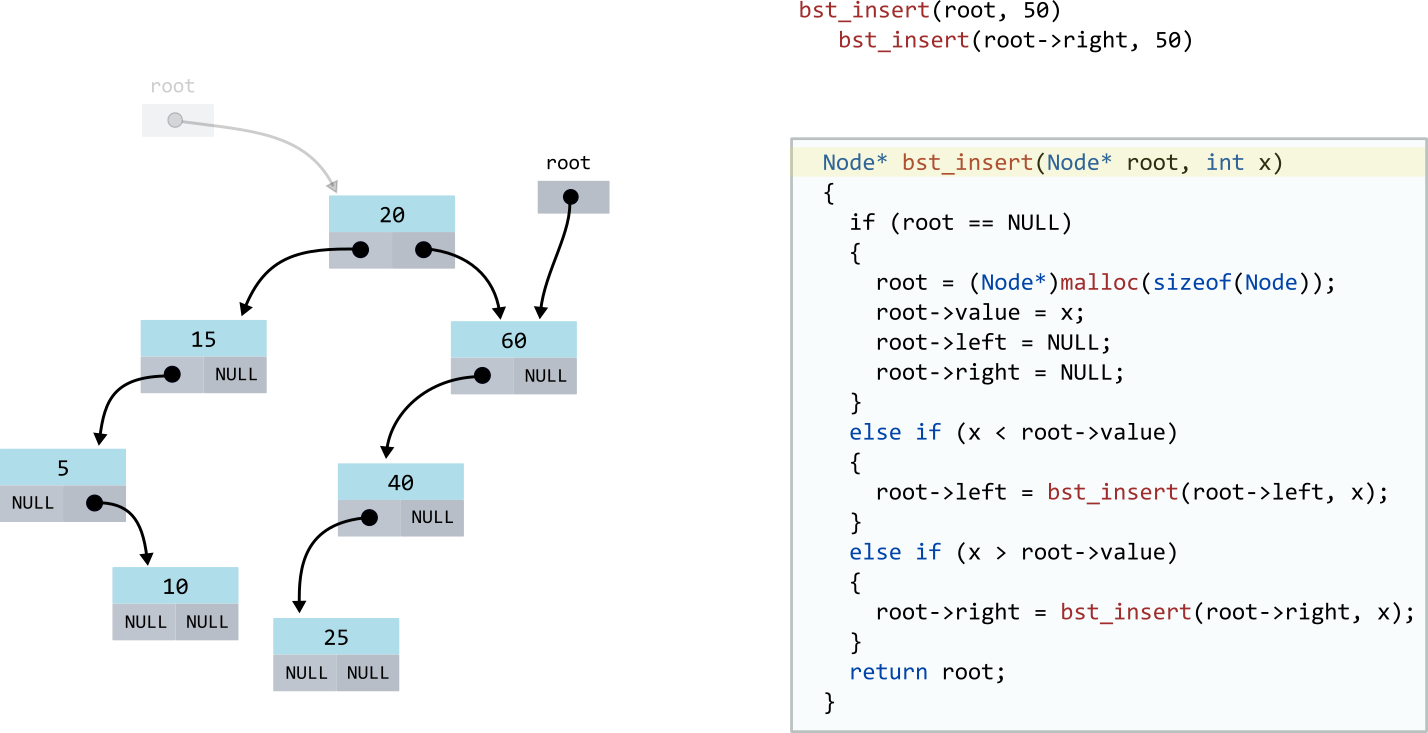
\includegraphics[width=\imageSizeMult\linewidth]{../images/codetree/codetree4.png}
\end{center}
\end{frame}

\begin{frame}[fragile]
\frametitle{Добавление элемента в бинарное дерево поиска}
\begin{center}
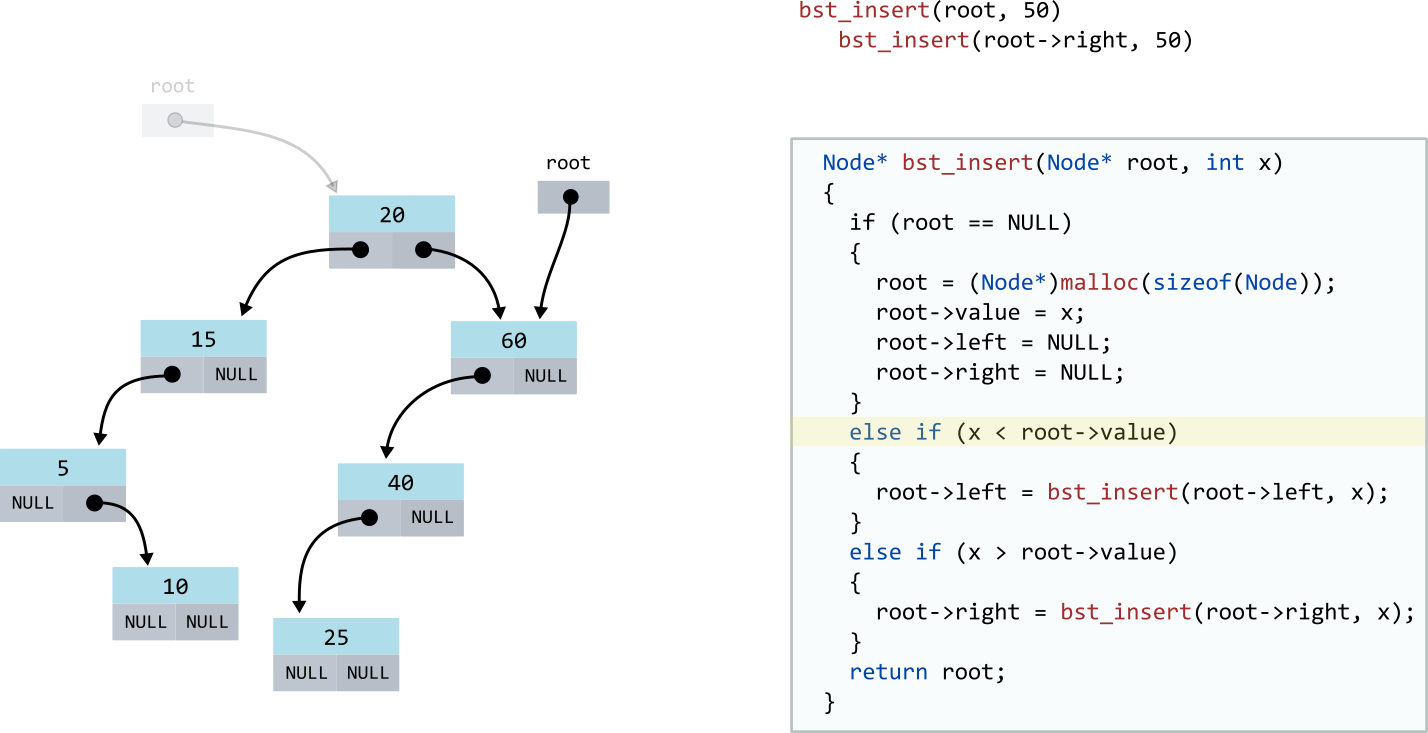
\includegraphics[width=\imageSizeMult\linewidth]{../images/codetree/codetree5.png}
\end{center}
\end{frame}

\begin{frame}[fragile]
\frametitle{Добавление элемента в бинарное дерево поиска}
\begin{center}
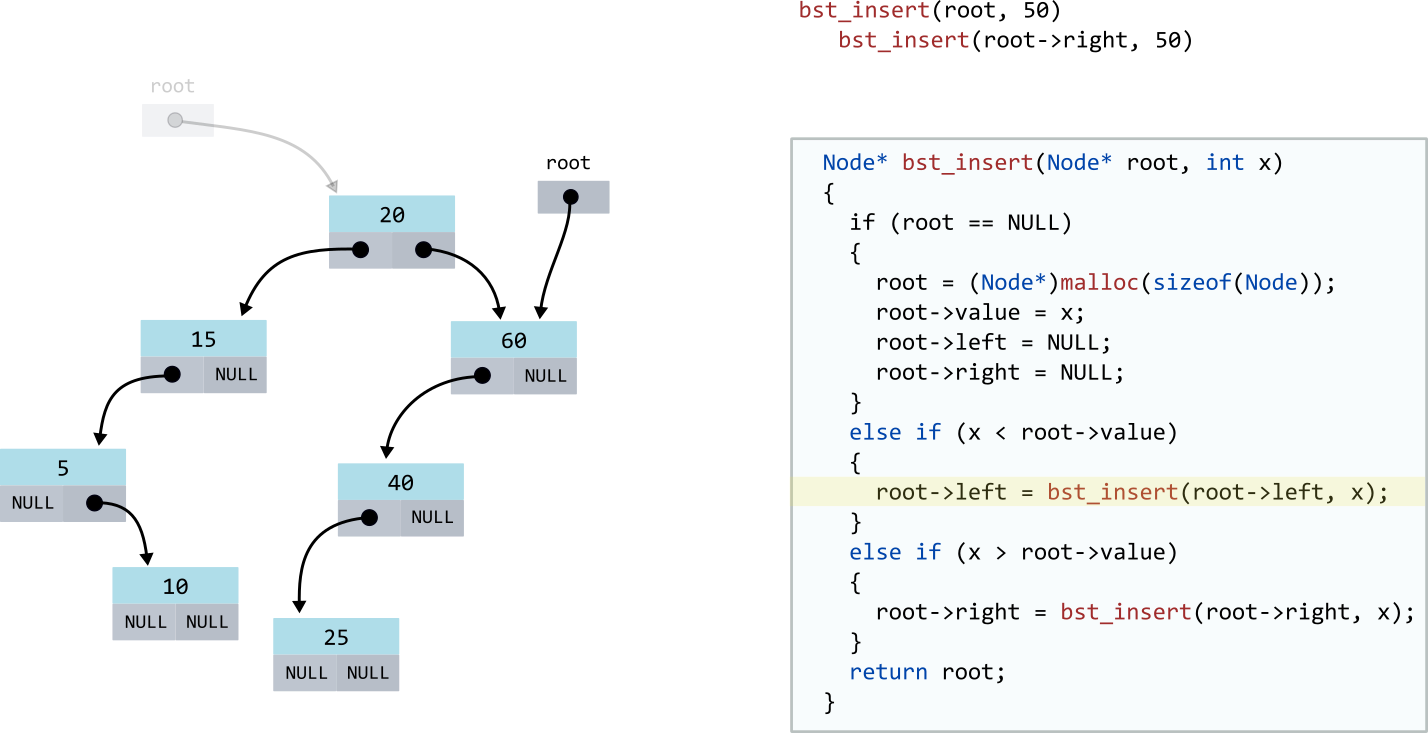
\includegraphics[width=\imageSizeMult\linewidth]{../images/codetree/codetree6.png}
\end{center}
\end{frame}

\begin{frame}[fragile]
\frametitle{Добавление элемента в бинарное дерево поиска}
\begin{center}
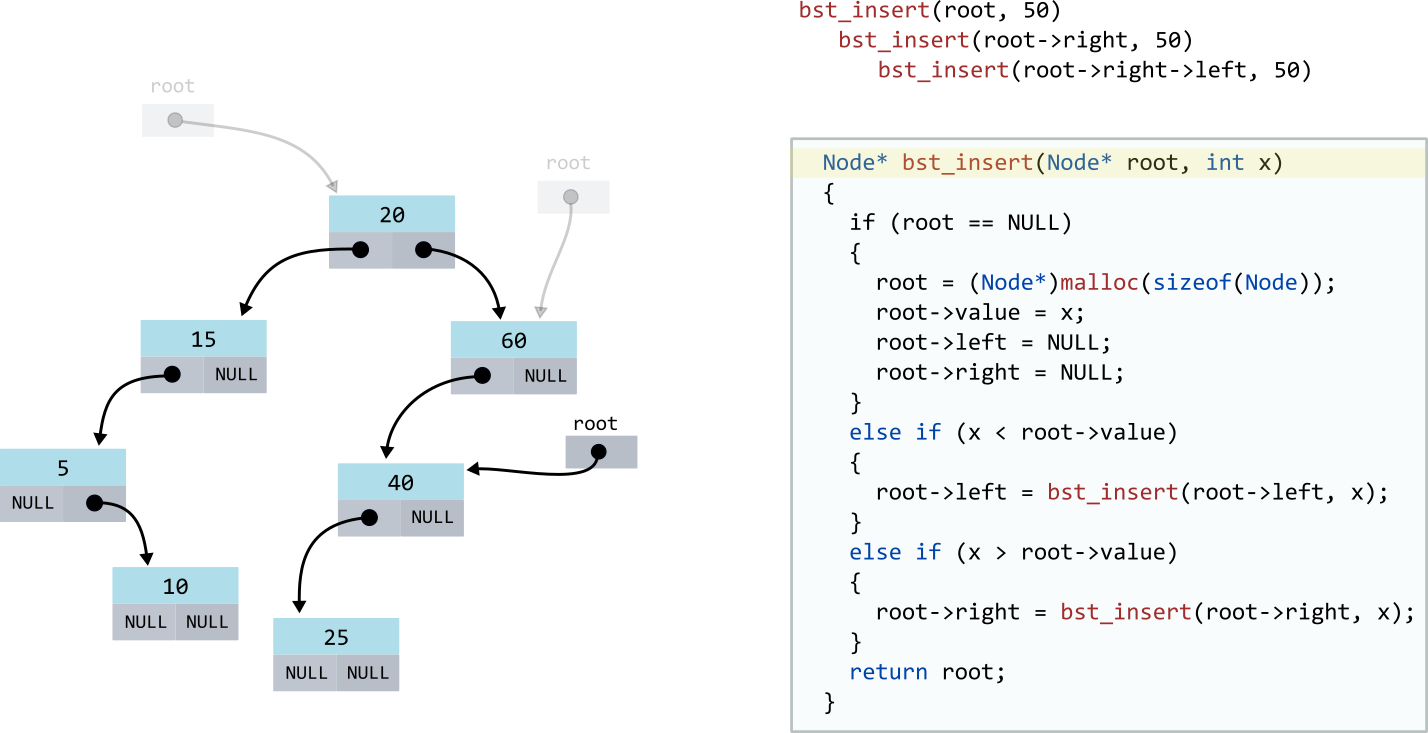
\includegraphics[width=\imageSizeMult\linewidth]{../images/codetree/codetree7.png}
\end{center}
\end{frame}

\begin{frame}[fragile]
\frametitle{Добавление элемента в бинарное дерево поиска}
\begin{center}
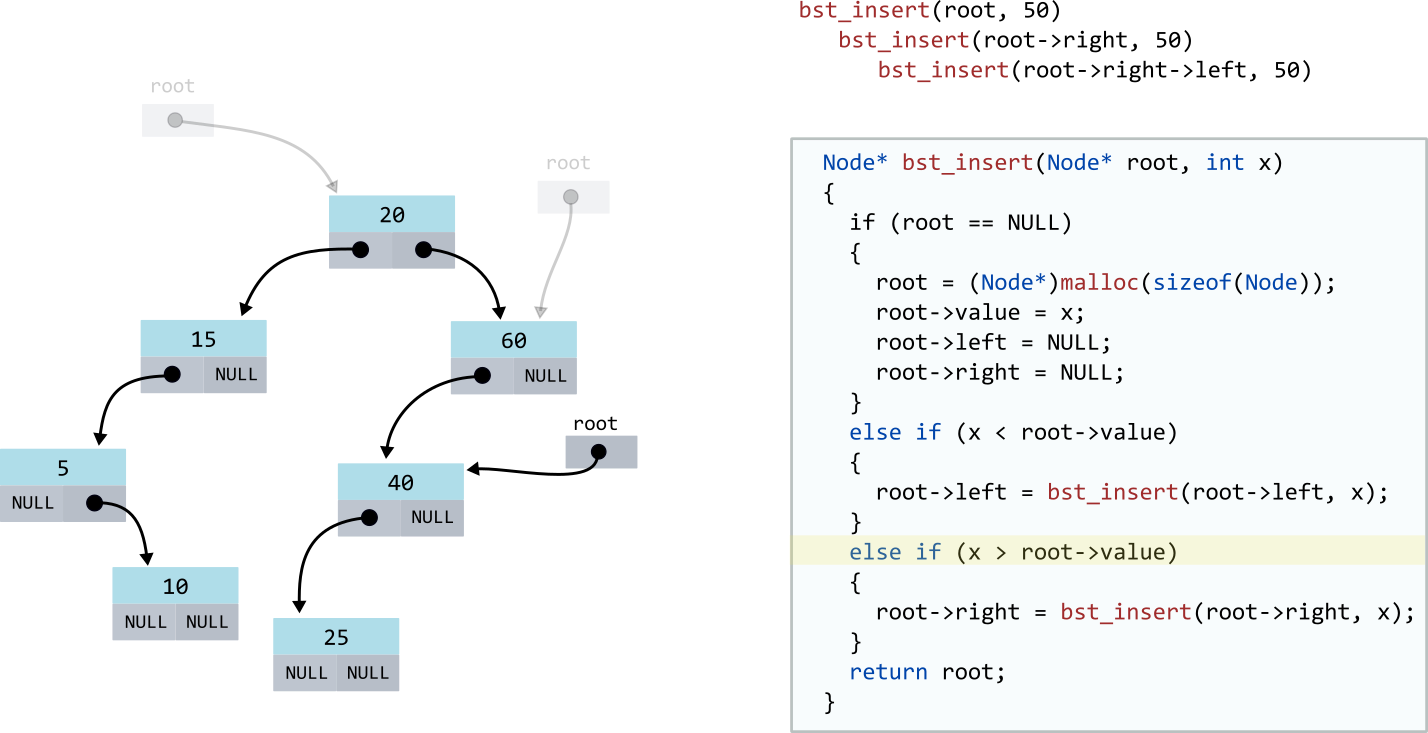
\includegraphics[width=\imageSizeMult\linewidth]{../images/codetree/codetree8.png}
\end{center}
\end{frame}

\begin{frame}[fragile]
\frametitle{Добавление элемента в бинарное дерево поиска}
\begin{center}
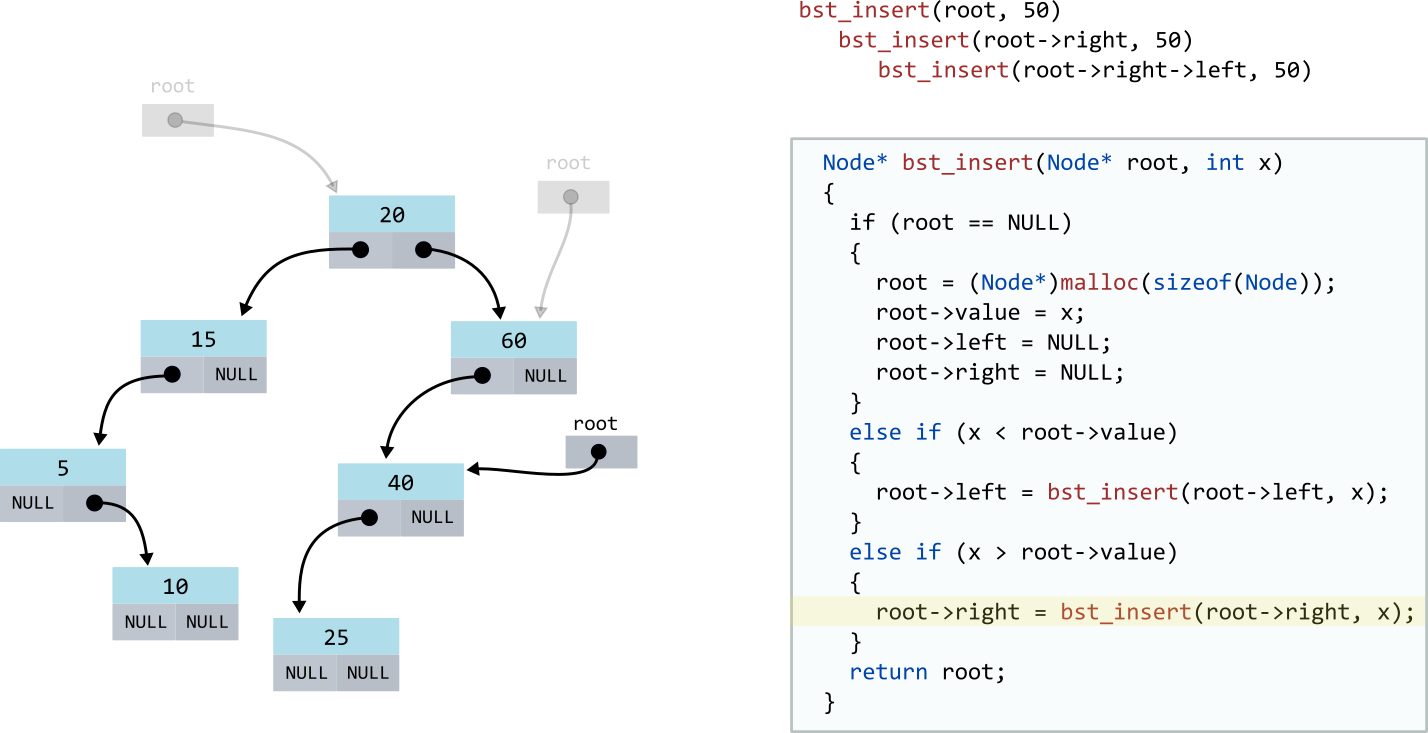
\includegraphics[width=\imageSizeMult\linewidth]{../images/codetree/codetree9.png}
\end{center}
\end{frame}

\begin{frame}[fragile]
\frametitle{Добавление элемента в бинарное дерево поиска}
\begin{center}
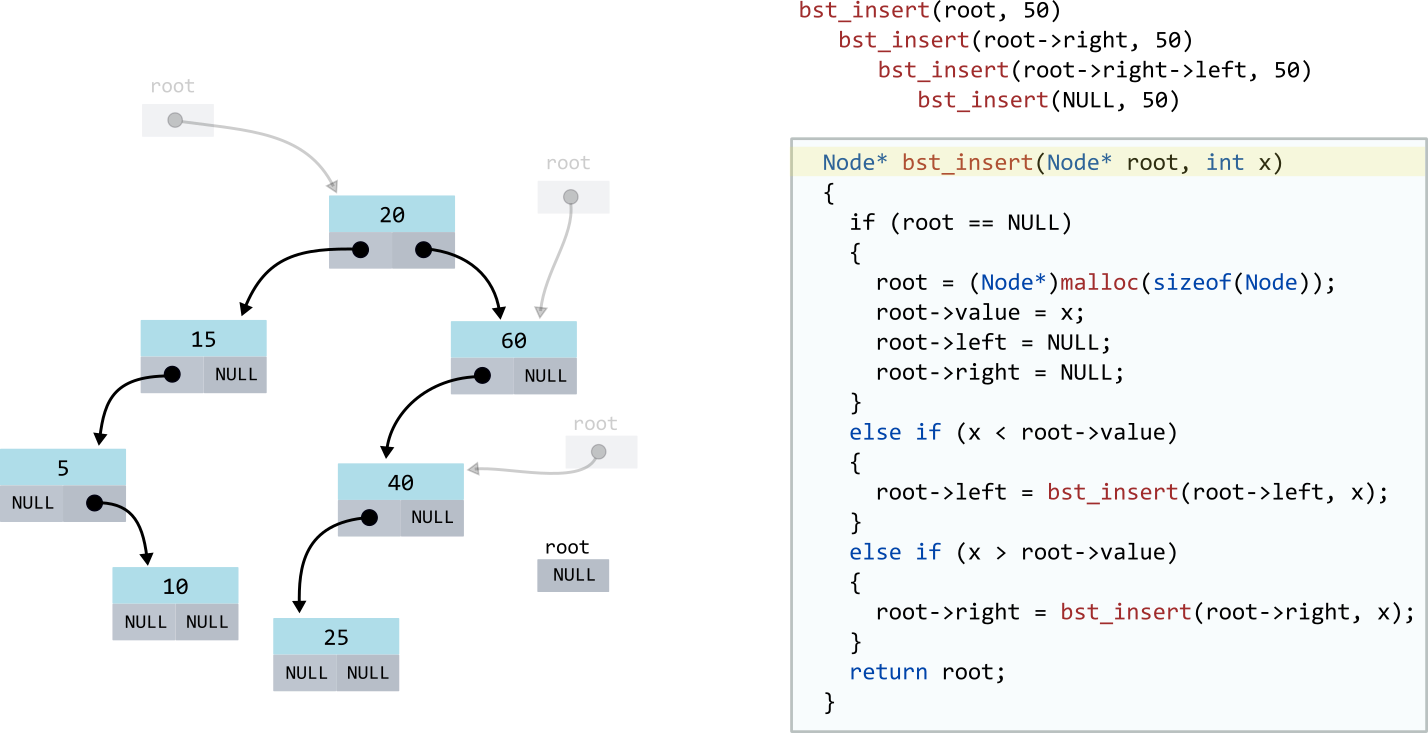
\includegraphics[width=\imageSizeMult\linewidth]{../images/codetree/codetree10.png}
\end{center}
\end{frame}

\begin{frame}[fragile]
\frametitle{Добавление элемента в бинарное дерево поиска}
\begin{center}
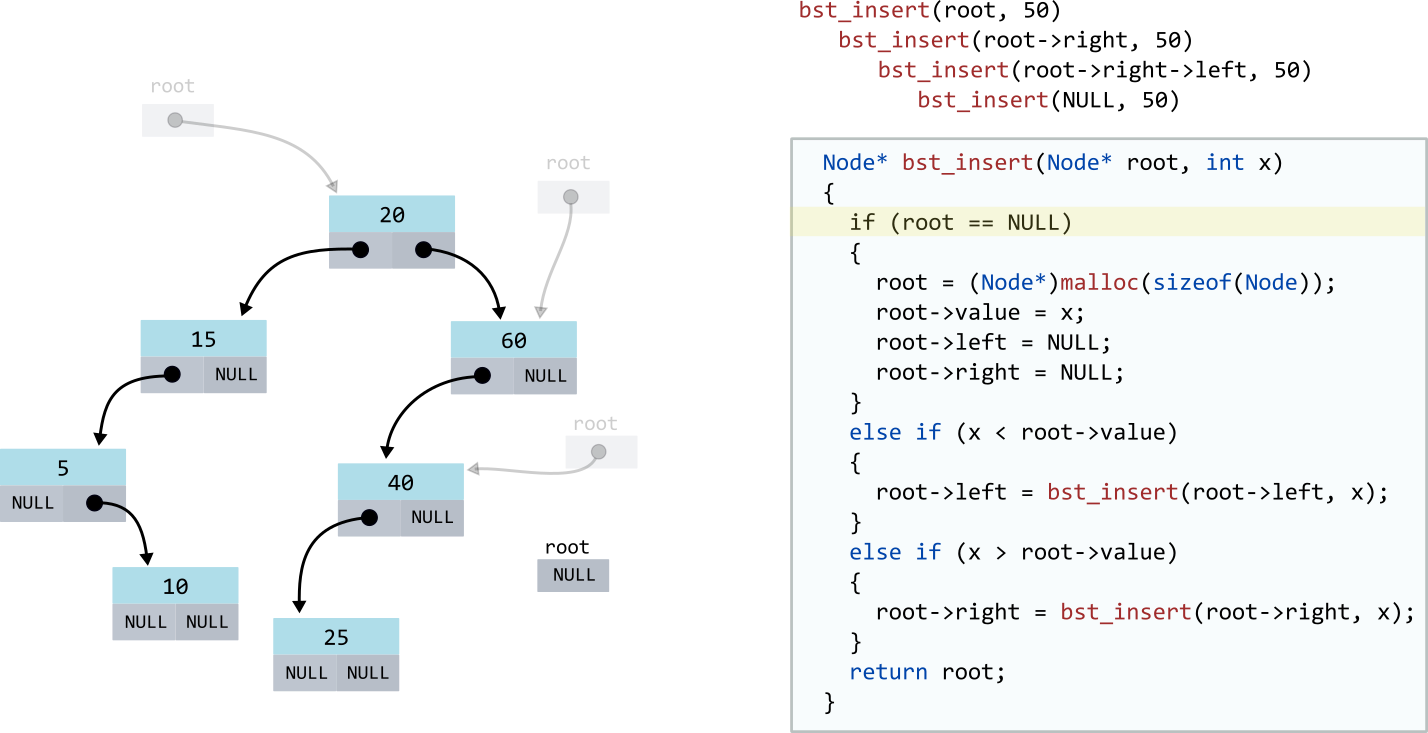
\includegraphics[width=\imageSizeMult\linewidth]{../images/codetree/codetree11.png}
\end{center}
\end{frame}

\begin{frame}[fragile]
\frametitle{Добавление элемента в бинарное дерево поиска}
\begin{center}
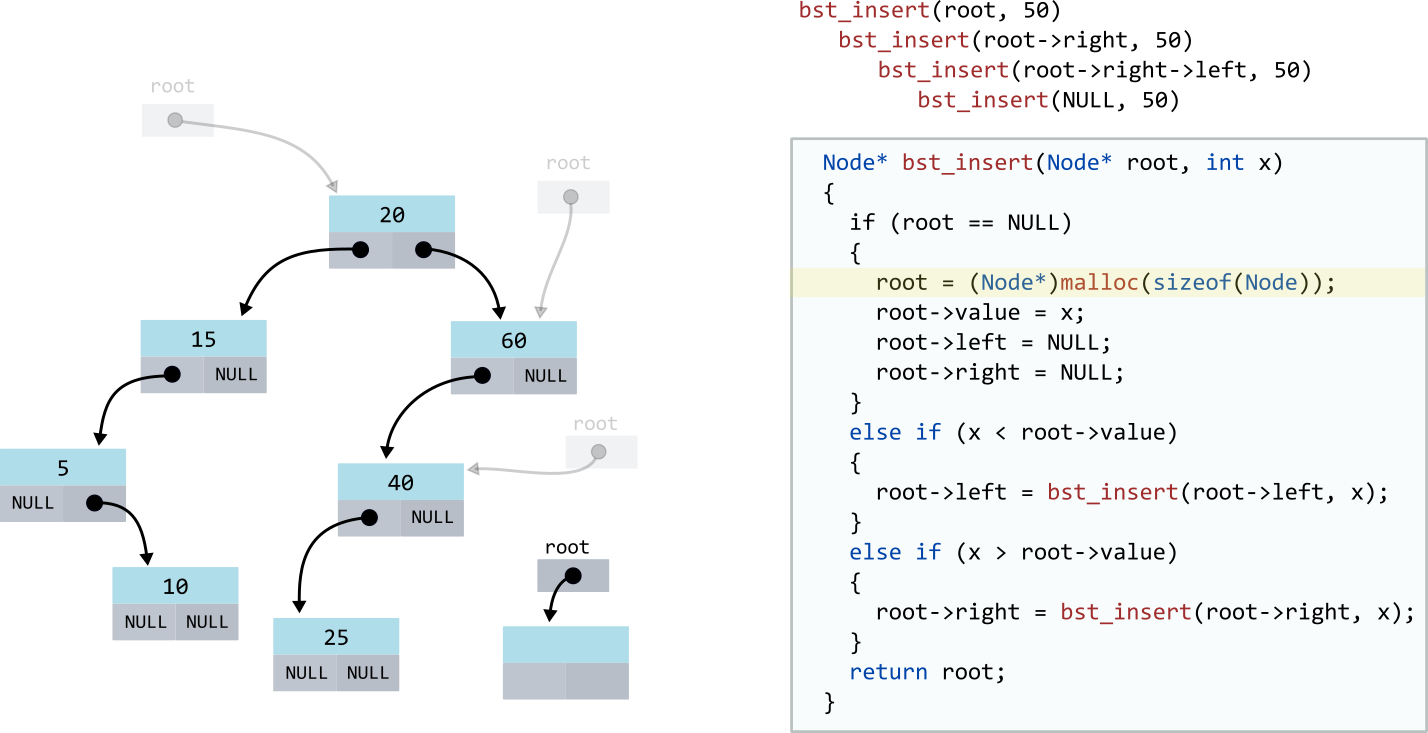
\includegraphics[width=\imageSizeMult\linewidth]{../images/codetree/codetree12.png}
\end{center}
\end{frame}

\begin{frame}[fragile]
\frametitle{Добавление элемента в бинарное дерево поиска}
\begin{center}
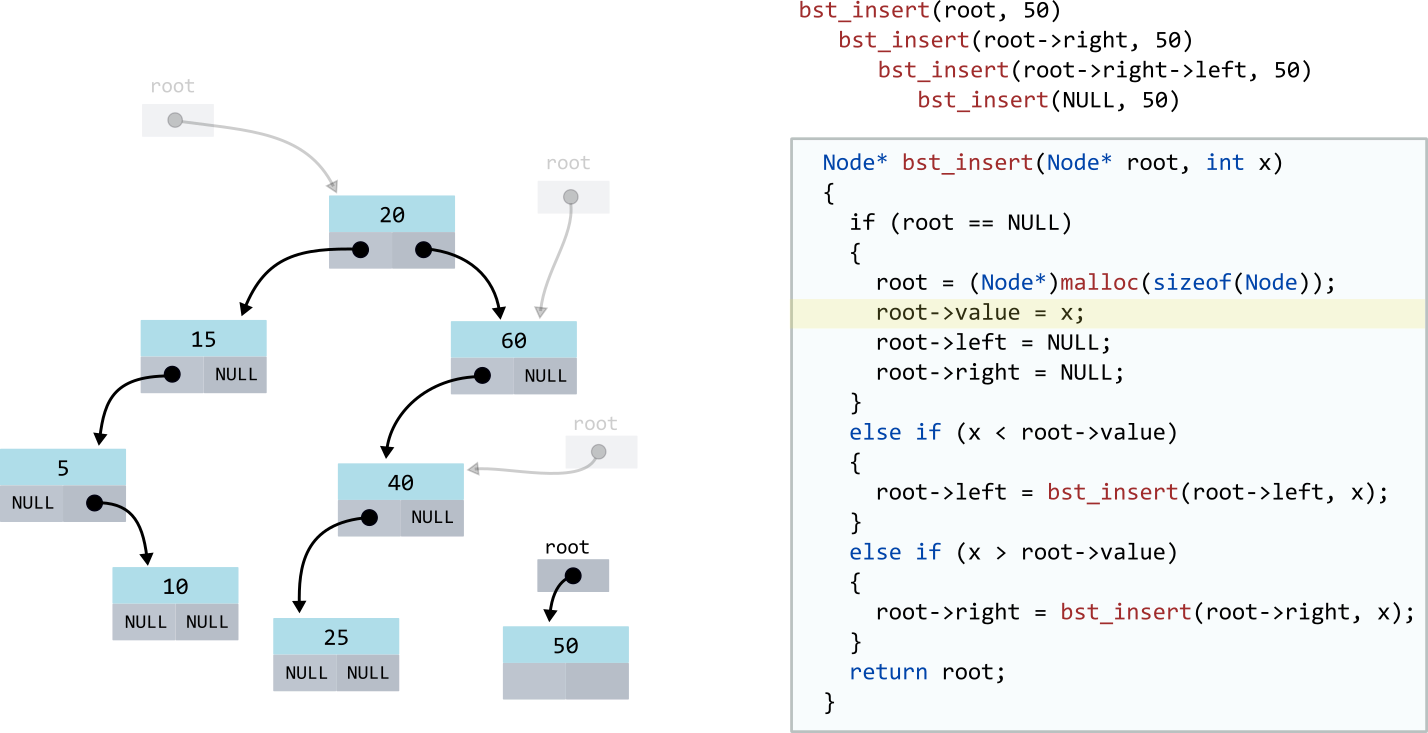
\includegraphics[width=\imageSizeMult\linewidth]{../images/codetree/codetree13.png}
\end{center}
\end{frame}

\begin{frame}[fragile]
\frametitle{Добавление элемента в бинарное дерево поиска}
\begin{center}
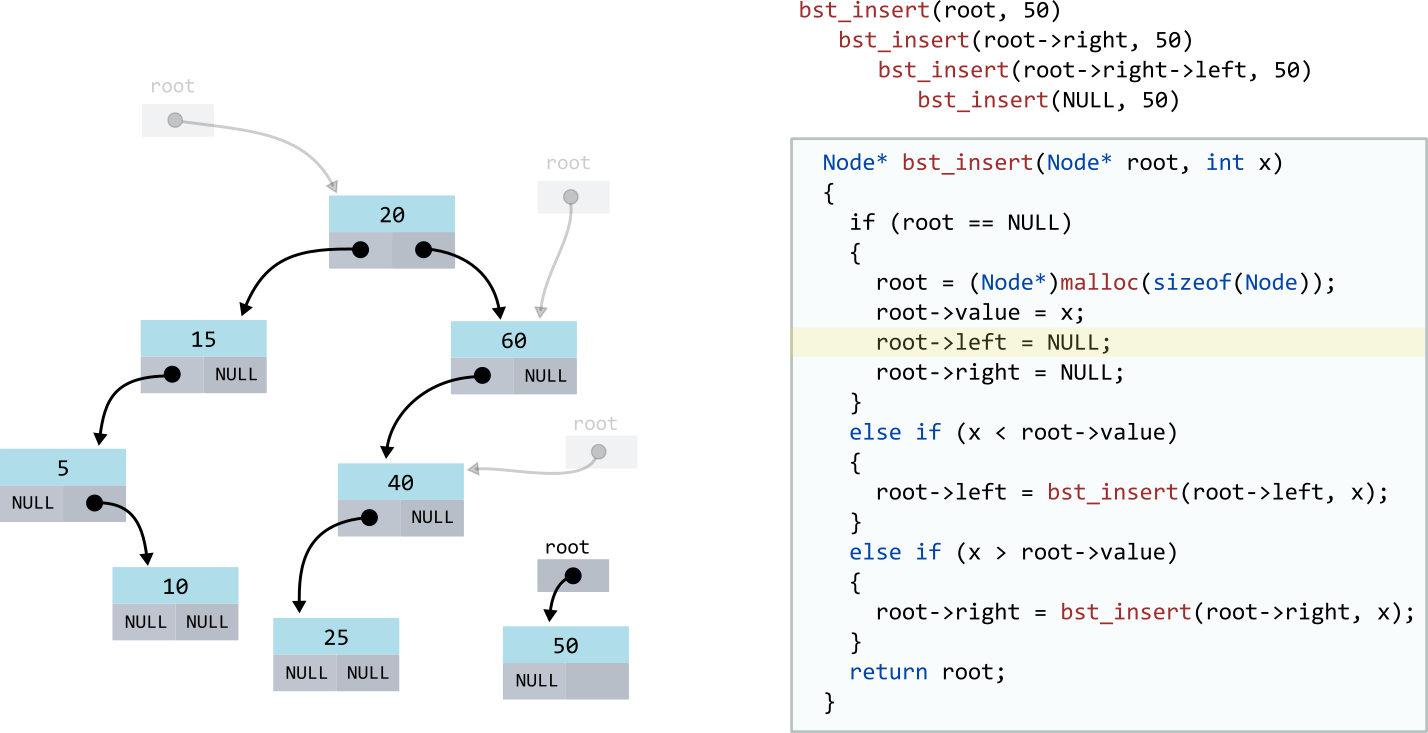
\includegraphics[width=\imageSizeMult\linewidth]{../images/codetree/codetree14.png}
\end{center}
\end{frame}

\begin{frame}[fragile]
\frametitle{Добавление элемента в бинарное дерево поиска}
\begin{center}
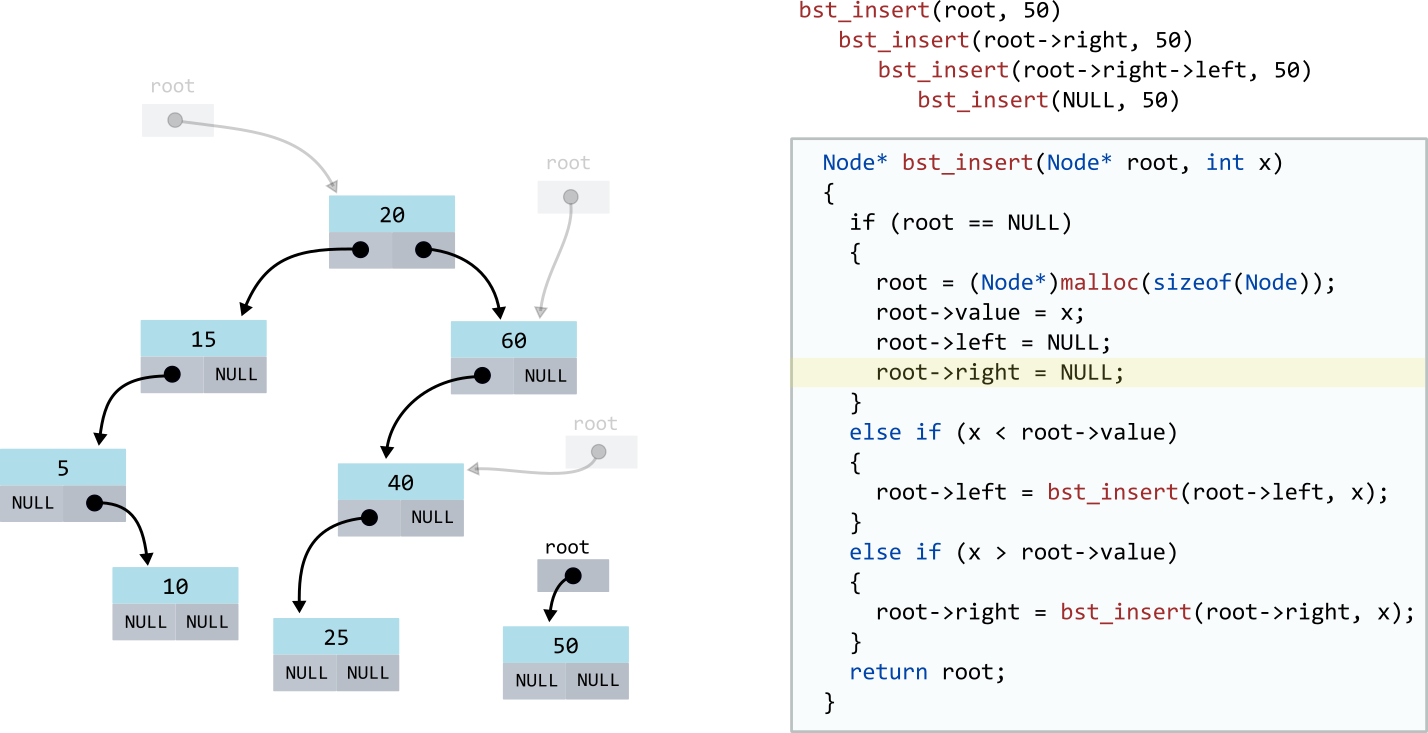
\includegraphics[width=\imageSizeMult\linewidth]{../images/codetree/codetree15.png}
\end{center}
\end{frame}

\begin{frame}[fragile]
\frametitle{Добавление элемента в бинарное дерево поиска}
\begin{center}
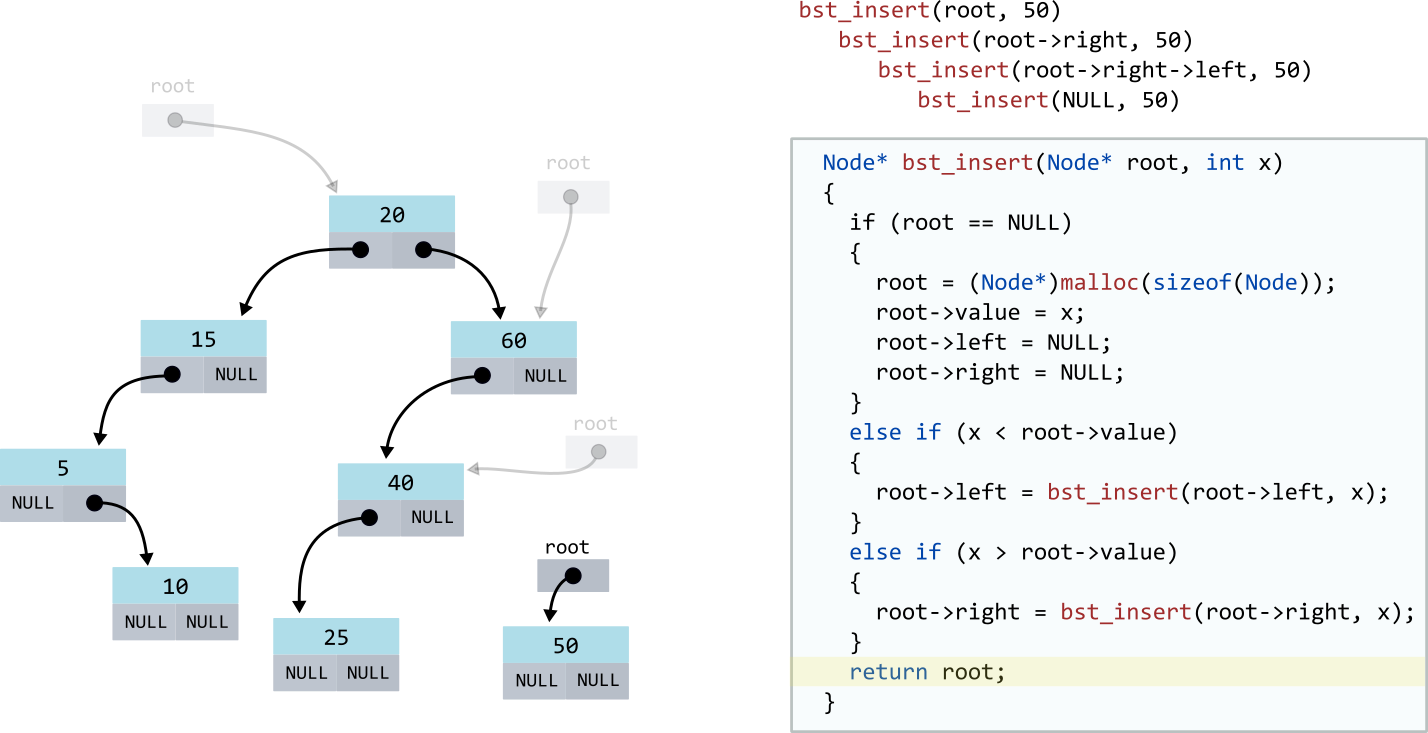
\includegraphics[width=\imageSizeMult\linewidth]{../images/codetree/codetree16.png}
\end{center}
\end{frame}

\begin{frame}[fragile]
\frametitle{Добавление элемента в бинарное дерево поиска}
\begin{center}
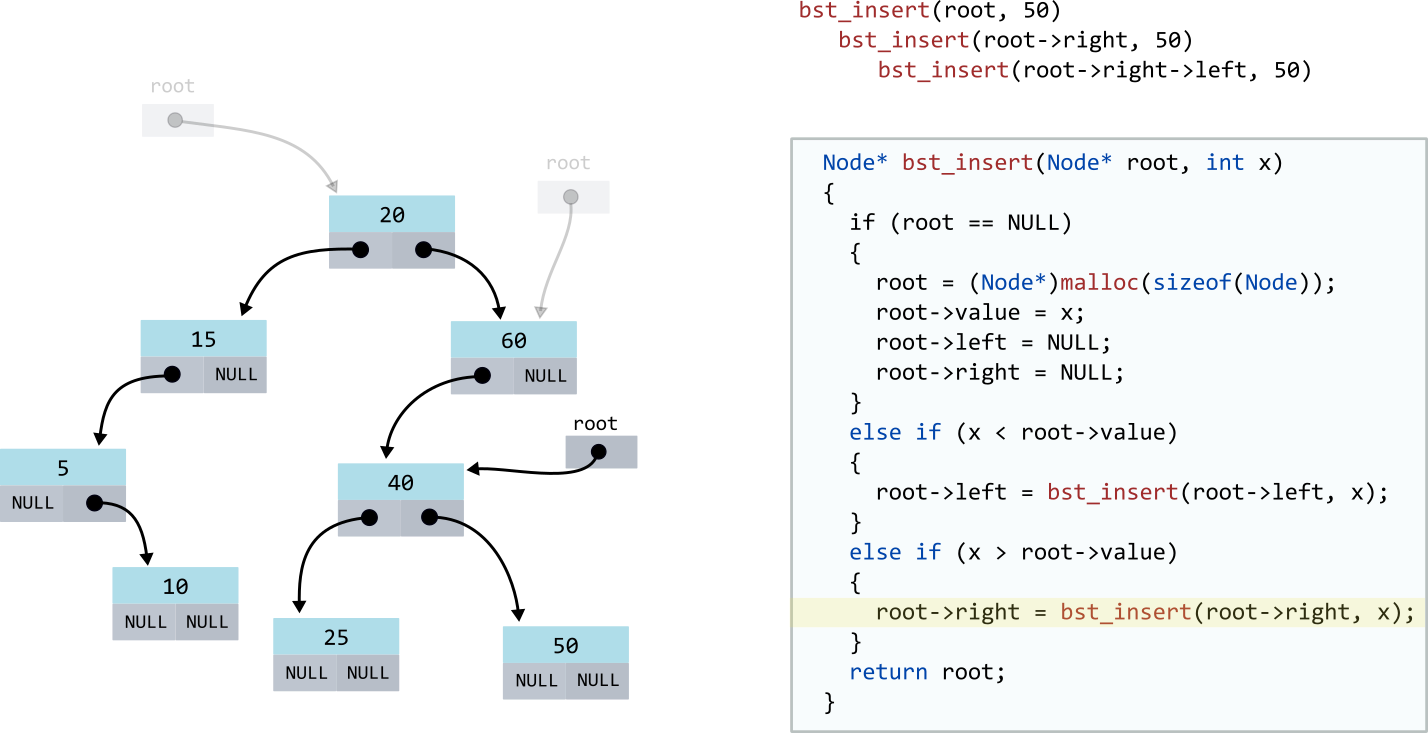
\includegraphics[width=\imageSizeMult\linewidth]{../images/codetree/codetree17.png}
\end{center}
\end{frame}

\begin{frame}[fragile]
\frametitle{Добавление элемента в бинарное дерево поиска}
\begin{center}
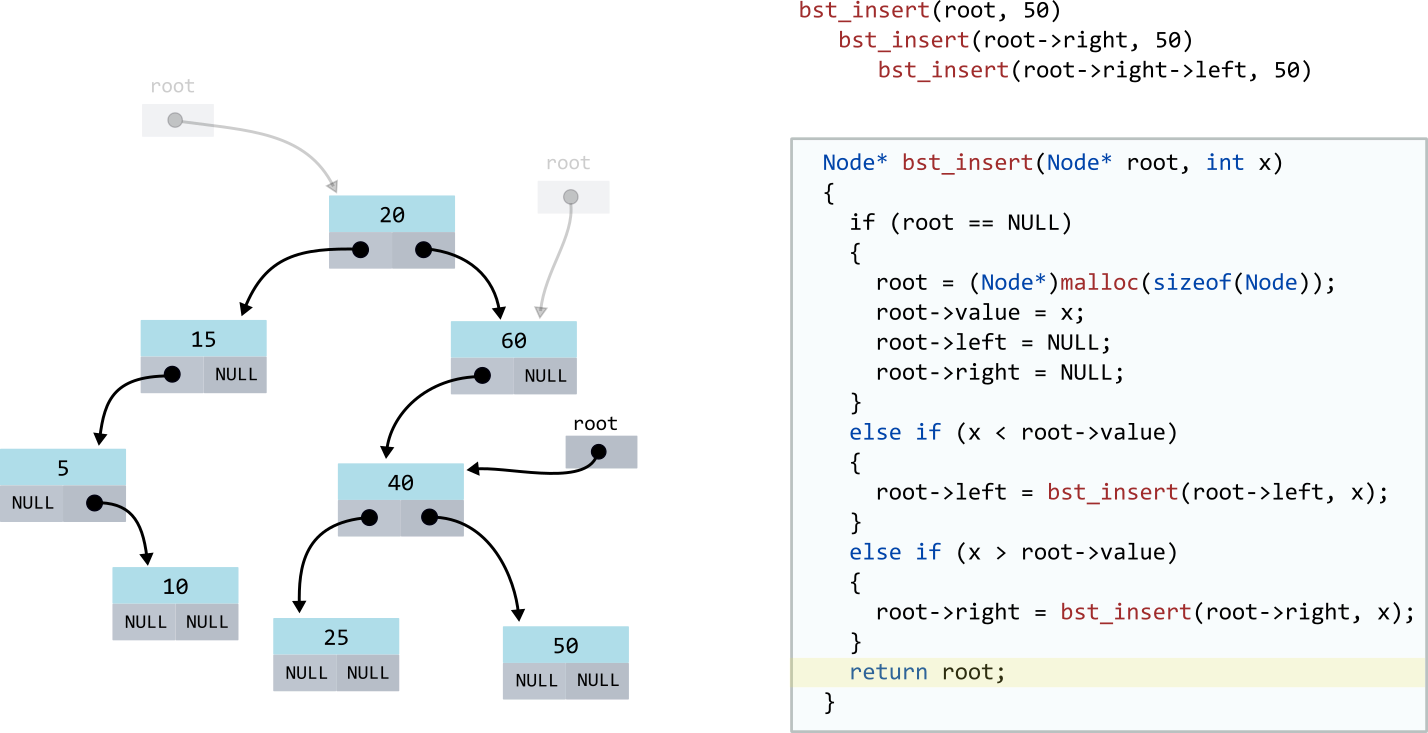
\includegraphics[width=\imageSizeMult\linewidth]{../images/codetree/codetree18.png}
\end{center}
\end{frame}

\begin{frame}[fragile]
\frametitle{Добавление элемента в бинарное дерево поиска}
\begin{center}
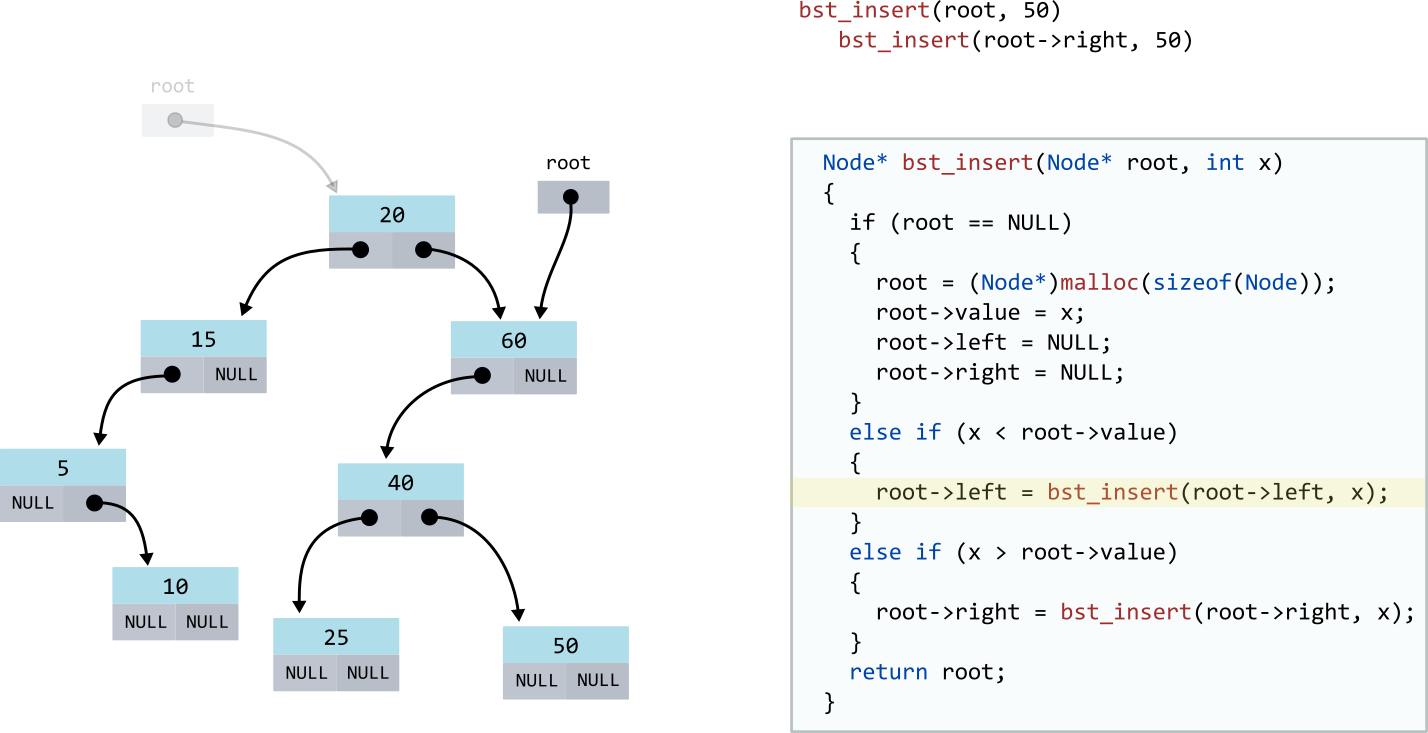
\includegraphics[width=\imageSizeMult\linewidth]{../images/codetree/codetree19.png}
\end{center}
\end{frame}

\begin{frame}[fragile]
\frametitle{Добавление элемента в бинарное дерево поиска}
\begin{center}
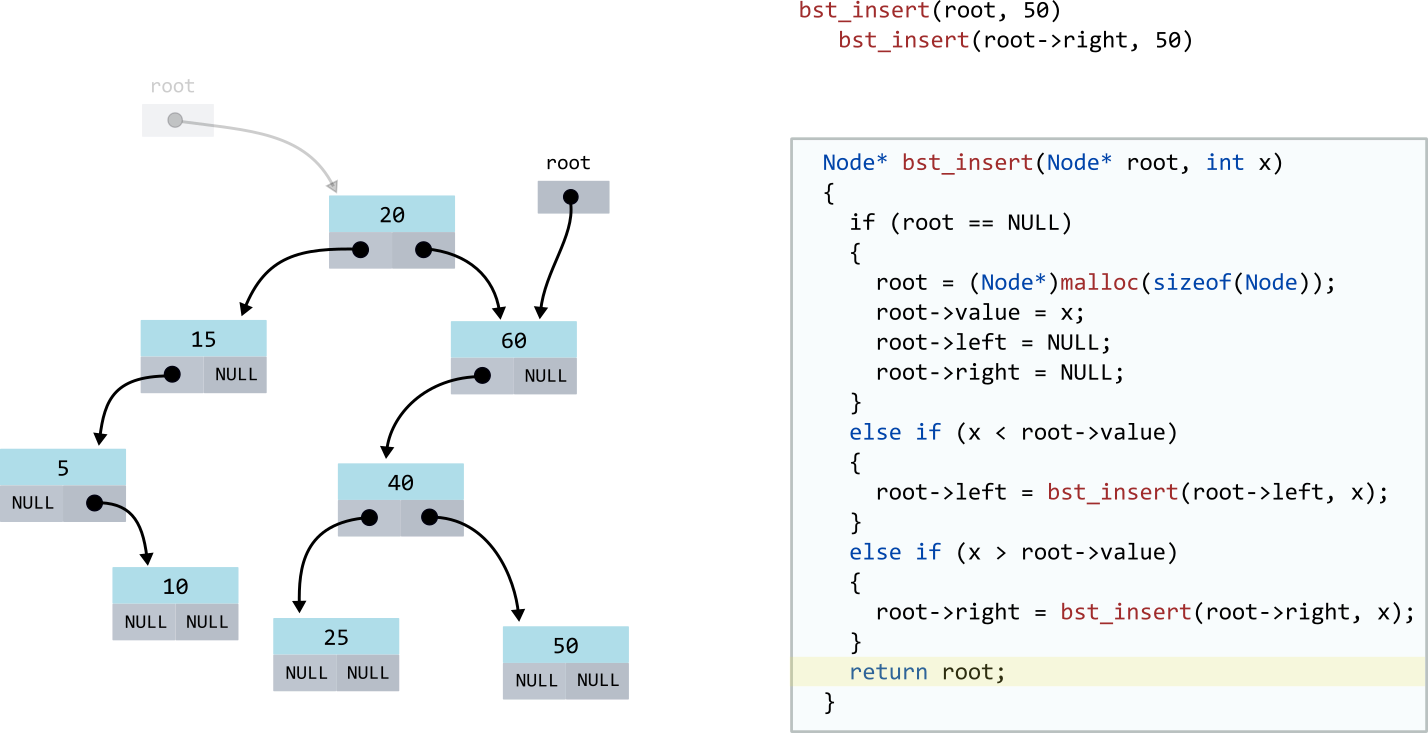
\includegraphics[width=\imageSizeMult\linewidth]{../images/codetree/codetree20.png}
\end{center}
\end{frame}

\begin{frame}[fragile]
\frametitle{Добавление элемента в бинарное дерево поиска}
\begin{center}
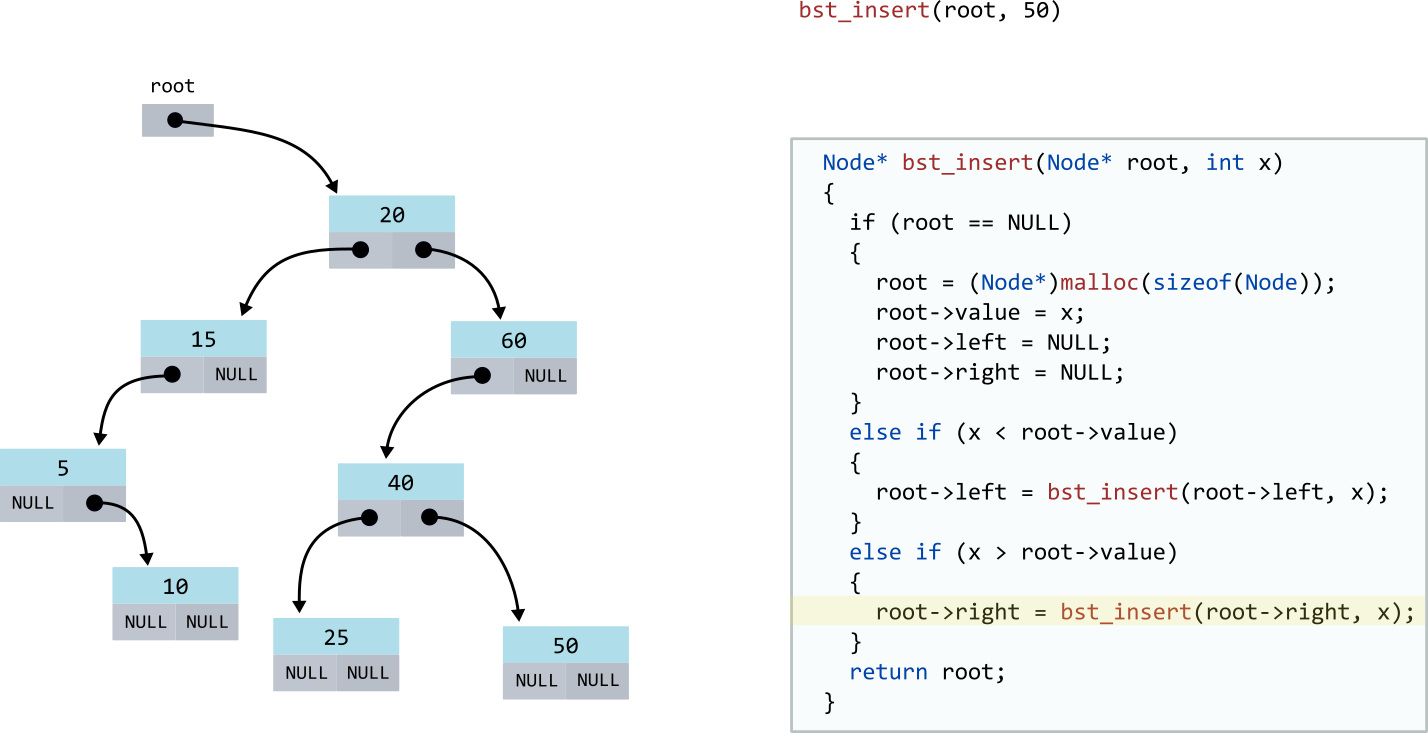
\includegraphics[width=\imageSizeMult\linewidth]{../images/codetree/codetree21.png}
\end{center}
\end{frame}

\begin{frame}[fragile]
\frametitle{Добавление элемента в бинарное дерево поиска}
\begin{center}
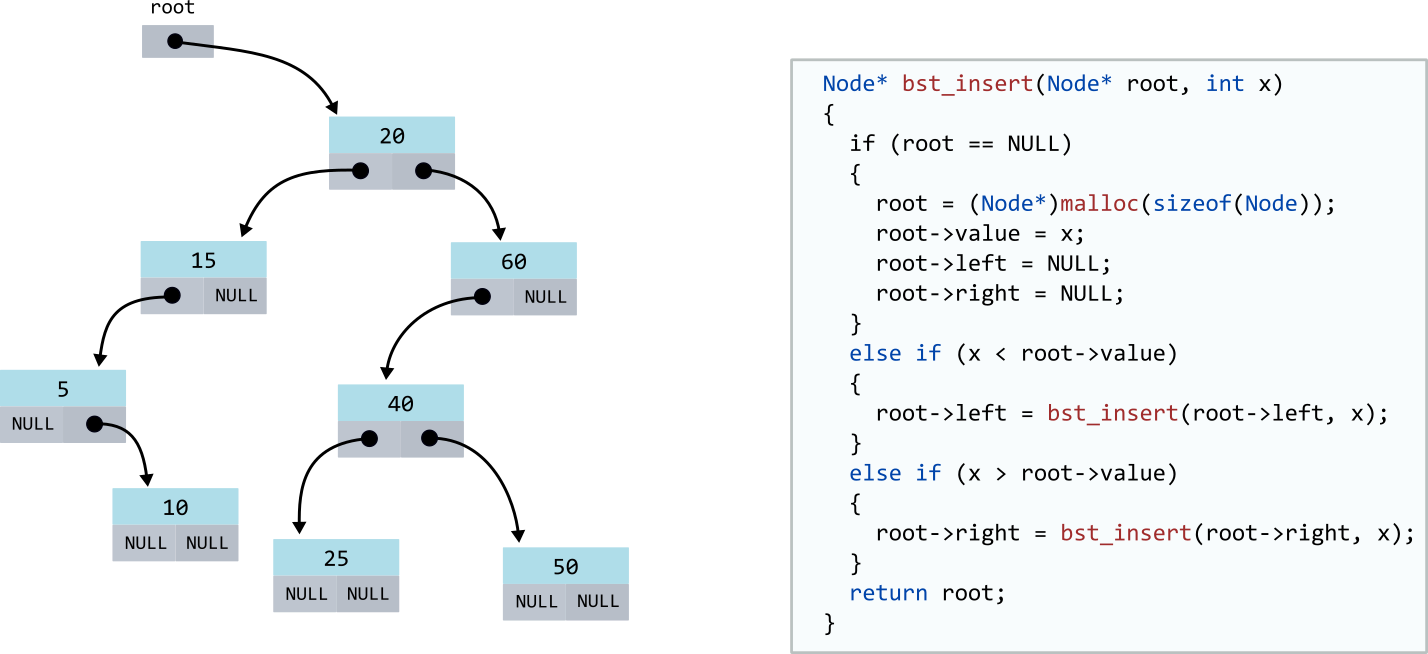
\includegraphics[width=\imageSizeMult\linewidth]{../images/codetree/codetree22.png}
\end{center}
\end{frame}


\end{document}
